\section{Beam Lifetime from Radial Oscillations} \label{eq:5.7}

In the preceding section I have argued that the likelihood that a stored electron will pass a given
 azimuth $s$ with a radial displacement between $x$ and $x + dx$ is distributed as a Gaussian error
 function -- namely as
\begin{align}\label{eq:5.116}
	w(x)dx = \dfrac{1}{\sqrt{2\pi}\sigma_x} \exp\left( -x^2/2\sigma_x^2 \right)dx,
\end{align}
with $\sigma_x$ a function of $s$. Such a distribution can clearly not be completely correct
since it has ``tails'' which extend to arbitrarily large positive and negative displacements while an actual stored beam must live in a vacuum chamber with a finite aperture! The probability
 distribution of Eq.~\eqref{eq:5.116} can be only an approximation which we may expect to be reasonably correct so long as the radial aperture is much larger than $\sigma_x$ everywhere around the ring.\\
Even when the aperture is large however, there may still be a significant effect from its finite extent. Sooner or later an electron will suffer a sufficiently large fluctuation in its emission of quanta to produce a radial displacement as large as the aperture limit. Then the electron will be lost by a collision with the edge of the vacuum chamber -- or whatever obstruction defines the limit of the aperture. Alternatively if we take into account the non linearities of the guide field, large amplitude oscillations may become unstable leading to the loss of the electron from the stored beam. It will be convenient for the present discussion to think in terms of an aperture
 that is limited by a physical obstruction. An extension of the discussion to a magnetic aperture
 limit is relatively straight-forward.\\
 So long as the chance of an electron being lost at the aperture limit is small -- by which we should mean that it is much less than 1 in a damping time -- the probability per unit time of getting lost is the same for all electrons. Then the loss rate from a stored beam will be proportional to the number $N$ of electrons present; and $N$ will therefore, decrease exponentially
 and with a time constant $\tau_q$ related to the loss rate by
\begin{align}
	\dfrac{1}{\tau_q} = - \dfrac{1}{N} \dfrac{dN}{dt}.
\end{align}
The number $\tau_q$ is usually referred to as the quantum lifetime of the stored beam.\\
A precise evaluation of the quantum lifetime for all conditions is a bit intricate. I shall therefore, show a way to compute it which is reasonably accurate only when the lifetime is long -- which is, after all, the condition of most interest for a storage ring. I shall first look at the lifetime due to lateral oscillations and then look later at the lifetime due to energy oscillations.\\
Let's think now of a somewhat over-simplified situation in which we imagine that only the radial betatron oscillations are excited -- ignoring for the moment the radial spread associated with the energy oscillations. We saw in Section~\ref{sec:2.6} that in the absence of radiation effects the betatron oscillations of an electron sweep out a band between the envelope limits
 $X(s) = a\sqrt{\beta(s)}$ -- recall Fig.\ref{fig:fig12}. When we include quantum effects and radiation
 damping, the ``invariant'' amplitude factor $a$ of any particular electron wanders up and down in a random way. The time scale of the variations of $a$ is however, rather slow -- that is, much
larger than the revolution time -- so we may think that the electron continuously sweeps out a radial band whose envelope is slowly varying.\\
Suppose now that there is at some azimuth, say $s_1$, an obstruction which defines an aperture
 limit of the ring. By that I mean that as the invariant amplitude $a$ is varied, the envelope $X(s)$ will first encounter an obstruction at $s_1$. See Fig.~\ref{fig:fig46}. All losses will occur at $s_1$ and we need only consider the radial distribution at this azimuth.
\begin{figure}[!htb]
	\centering
	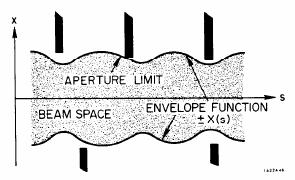
\includegraphics[width=0.8\linewidth]{./Figuras/fig46.jpeg}
	\caption{Radial aperture limit.}
	\label{fig:fig46}
\end{figure}
We have seen in Section~\ref{sec:2.7} that the radial displacement on successive passages of any chosen azimuth varies with time as
\begin{align}
	x = a \sqrt{\beta_1} \cos\omega t.
\end{align}
As we did in Section\ref{sec:5.3} for the energy oscillations we may take the square of the
amplitude factor as a measure of the ``effective energy'' of the oscillations. Let's define
\begin{align}
	W = a^2 \beta_1.
\end{align}
Quantum effects and radiation damping produce slowly varying fluctuations in $W$. The same arguments made in Section~\ref{sec:5.3} can be used again to show that -- in the absence of any aperture limit -- the electrons in a beam will have a distribution of $W$'s according to (see Eq.~\eqref{eq:5.62})
\begin{align}\label{eq:5.120}
	h(W) = \dfrac{N}{\mean{W}}\exp(-W/\mean{W}),
\end{align}
where the mean value $\mean{W}$ is equal to $2\sigma_x^2$ (the function $h(W)$ is defined such
that the number of electrons with ``oscillation energy'' between $W$ and $W + dW$ is $h(W)dW$). The function $h(W)$ is shown by the solid curve in Fig.~\ref{fig:fig47}.
\begin{figure}[!htb]
	\centering
	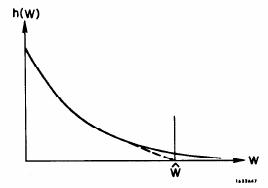
\includegraphics[width=0.8\linewidth]{./Figuras/fig47.jpeg}
	\caption{Distribution of oscillation energies.}
	\label{fig:fig47}
\end{figure}
Now consider what happens when there is an aperture limit that removes any electron for which $W$ exceeds some limiting value $\hat{W}$ -- which we may call ``$W$-peak''. There can be no electrons with $W > \hat{W}$, so the actual distribution $h(W)$ must change for large $W$ to correspond to something like the broken line curve in Fig.~\ref{fig:fig47}. We may think about what is happening in the following way. The quantum effects are continually trying to fill in the ideal distribution by a ``diffusion'' of electrons from the region of small $W$ into the region of large $W$. But each time an electron reaches $\hat{W}$ it is ``wiped off'', so there is a continuous loss out of the tail of the distribution. I would like now to make an estimate of this loss rate.\\
We may make a rough estimate in the following way. We have said that there is a characteristic
 ``relaxation time'' for the quantum fluctuations equal to the damping time constant $\tau_x$. We may guess that there is an ``attempt'' to fill in the tail of the ideal distribution once each damping time. Then the number of electrons lost in each damping time will be equal to the number of electrons in the ideal distribution with $W > \hat{W}$. That number is
\begin{align}
	N(>\hat{W}) = \int_{\hat{W}}^\infty h(W) dW = N \exp(-\hat{W}/\mean{W}).
\end{align}
The electron loss rate will then be estimated by
\begin{align}
	- \dfrac{dN}{dt} \approx \dfrac{N}{\tau_x} \exp(-\hat{W}/\mean{W}),
\end{align}
which would give a quantum lifetime of
\begin{align}\label{eq:5.123}
	\tau_q \approx \tau_x \exp(\hat{W}/\mean{W}).
\end{align}
We would estimate that the lifetime itself depends exponentially on $\hat{W}/\mean{W}$.\\
An exact calculation of $\tau_q$ requires setting up a diffusion equation for $h(W)$ and solving it numerically with the appropriate boundary conditions. I shall not attempt to do this but rather show how a good approximation to the exact result can be obtained.\\
Consider what would be happening in the neighborhood of some particular $W_0$ that is much greater than $\mean{W}$ if there were no aperture limit. The chance of finding any particular
 electron with $W > W_0$ in the ideal distribution is very small. We may expect that if an electron once gets into the tail ($W > W_0$) it is most likely to return rather quickly to the main body of the distribution -- being replaced in the tail by some other unfortunate electron. Consider now the flux of electrons passing through a small zone\footnote{We should think of passage through a ``zone'' so that we may ignore the microscopic fluctuations in the amplitude.} near $W_0$. The electrons which have been populating the tail will be passing to the left through this zone and an equal flux of electrons will (in the stationary state) be passing toward the right through the zone due to abnormal quantum fluctuations (we are neglecting the unlikely events in which an electron leaving the tail would have at that instant an abnormal fluctuation and reenter the tail of the distribution right away).\\
Let's estimate the flux of electrons coming out of the tail. When $W$ is large the ``normal'' energy fluctuations can be neglected in comparison with the rate of decrease of $W$ due to the damping. For any electron the damping gives
\begin{align}\label{eq:5.124}
	\dfrac{dW}{dt} = - \dfrac{2W}{\tau_x},
\end{align}
and the flux of electrons through $W_0$ due to the damping will be
\begin{align}\label{eq:5.125}
	\left\lbrace h(W) \dfrac{dW}{dt} \right\rbrace_{W_0} = \dfrac{2 W_0 h(W_0)}{\tau_x}.
\end{align}
In the absence of an aperture limit the net flux through any $W$ -- and past $W_0$ in particular
 -- must be zero so there would also be an outward flux of electrons quite equal to the inward flux of \eqref{eq:5.125}.\\
Now put in the aperture limit at $\hat{W}$. If it is sufficiently large, the main body of the distribution is little affected. The flux outward through $\hat{W}$ will be unchanged while the return flux will of course, be zero. We have that the flux of \eqref{eq:5.124}, evaluated at $W_0 = \hat{W}$, is also an estimate of the outward flux of lost electrons. The loss rate will be
\begin{align}
	-\dfrac{dN}{dt} = \dfrac{2\hat{W}h(\hat{W})}{\tau_x}.
\end{align}
Using Eq.~\eqref{eq:5.120} for $h(W)$ we obtain,
\begin{align}\label{eq:5.127}
	\tau_q = \dfrac{\tau_x}{2} \dfrac{\mean{W}}{W} \exp \left( \hat{W}/\mean{W} \right).
\end{align}
Remember that $\hat{W}$ and $\mean{W}$ are related to the limiting radial excursion permitted by the aperture (assumed to occur at some azimuth $s_1$) and the rms radial displacement at that azimuth by
\begin{align}
	\hat{W} = \left[ a^2 \beta(s_1) \right]_\text{Max}; && \mean{W} = 2\sigma_x^2(s_1),
\end{align}
with both numbers evaluated at the azimuthal position of the limiting aperture.\\
This result differs from the estimate in Eq.~\eqref{eq:5.123} by the factor $\mean{W}/2\hat{W}$ and gives, therefore, a lifetime smaller by a factor which might be typically 5 or 10. The discrepancy can be explained by arguing that the ``relaxation time'' is shorter by this factor for the population of the tail of the distribution than for the main body of it -- which is understandable since a large fluctuation has a better chance of dominating the radiation damping if it accumulates during a relatively short time span. Although Eq.~\eqref{eq:5.127} was derived by making some approximations whose quantitative significance we have not tried to estimate, the same result has been obtained by more sophisticated -- although still approximate -- techniques (see \cite{5}, \cite{15}).\\
In our derivation of the quantum lifetime we have assumed that the radial fluctuations were due solely to betatron oscillations. As we have seen in Section~\ref{sec:5.5} however, the radial beam spread has contributions from both the betatron and energy oscillations. And the analysis is complicated by the fact that the two components have different damping time constants. I shall not attempt to refine the calculation but settle for the following comments. The two damping time constants are not very different -- usually within a factor of two of each other. It is then clear that Eq.~\eqref{eq:5.125} will give a reasonable approximation if we use for $\sigma_x^2$ the total mean-square beam spread and for $\tau_x$ some value between the betatron and synchrotron damping time constants. Or alternatively we may get a ``safe'' estimate of $\tau_q$ -- that is a lower limit -- by using for $\tau_x$ the smaller of the two time constants.\\
The quantum lifetime increases approximately exponentially with the square of the limiting radial excursion -- an exceedingly rapid variation. There is then, a rather precise criterion
 for the aperture required. If the aperture is just a little bit too small the lifetime will be disastrously short, but if it is a little larger than necessary the lifetime will be astronomically large and will be of no consequence\footnote{Since other loss mechanisms
 will then dominate.}. The ``critical'' aperture limit occurs at about
\begin{align}
	\dfrac{|x_\text{max}|}{\rho_x} = 6\sigma_x.
\end{align}
which gives $\hat{W}/\mean{W} \approx 18$ and from Eq.~\eqref{eq:5.120},
\begin{align}
	\tau_q = \dfrac{\tau_x}{36} e^{18} \approx 1.5 \times 10^6 \tau_x.
\end{align}
Since $\tau_x$ is typically about 0.1 sec, the critical aperture gives a quantum lifetime
of about one day. Other effects such as gas scattering usually give lifetimes of several hours and the filling time (time to store an operating beam) is generally a fraction of an hour, so a quantum lifetime of one day is quite ``safe''. We can understand the ``rule-of-thumb'' that the full aperture must be at least 12 times the standard deviation $\sigma_x$ of the radial distribution. A similar rule clearly holds for the vertical aperture.
